\graphicspath{{sec03/images/}{sec03/code/}}
\lstset{inputpath=sec03/code/}
\subsection{Common graphs}
\begin{frame}{Graph example 1\magicPage}\relax
\twocolImg{
\lstinputlisting[linerange={9-10, 16-27}, basicstyle=\tt\tiny]{graphSample.tex}
}{graphSample}
 
 You can write \ccol{below=of <label>} to have a relative coordinate
 
\end{frame}

\begin{frame}{Chain example\magicPage}\relax
     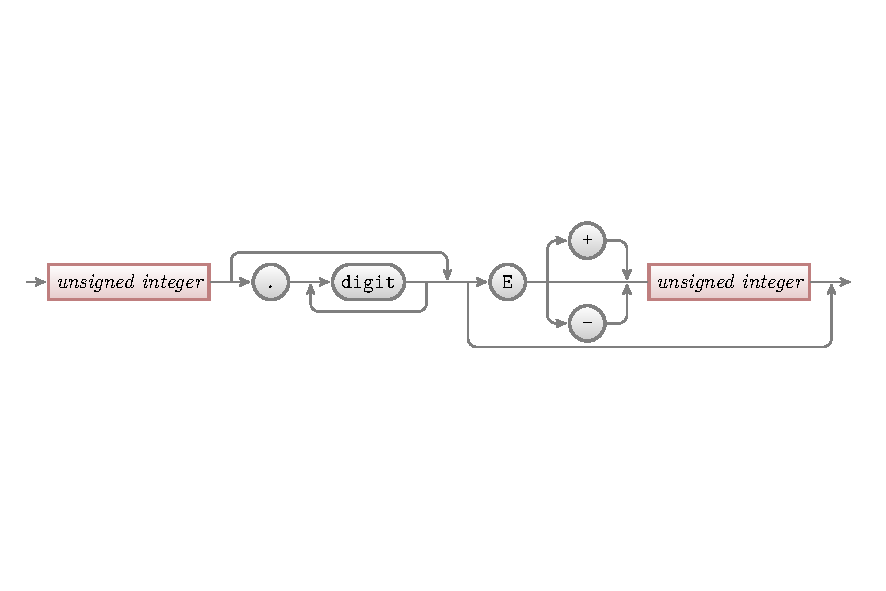
\includegraphics[width=\textwidth]{chainSample}
     
     \skfootnote{\tikzc{I.5}[69]}
\end{frame}

\subsection{Trees}

\begin{frame}{Tree}

\twocolImg{
\lstinputlisting[linerange={9-9, 16-25}, basicstyle=\tt\tiny]{treeSample.tex}
}{treeSample}

We use \ccol\node\ and \ccol{child}.

\ccol{sibling distance} option provides a horizontal distance between nodes
     
\end{frame}
